\begin{figure}[h!]
  \centering    
    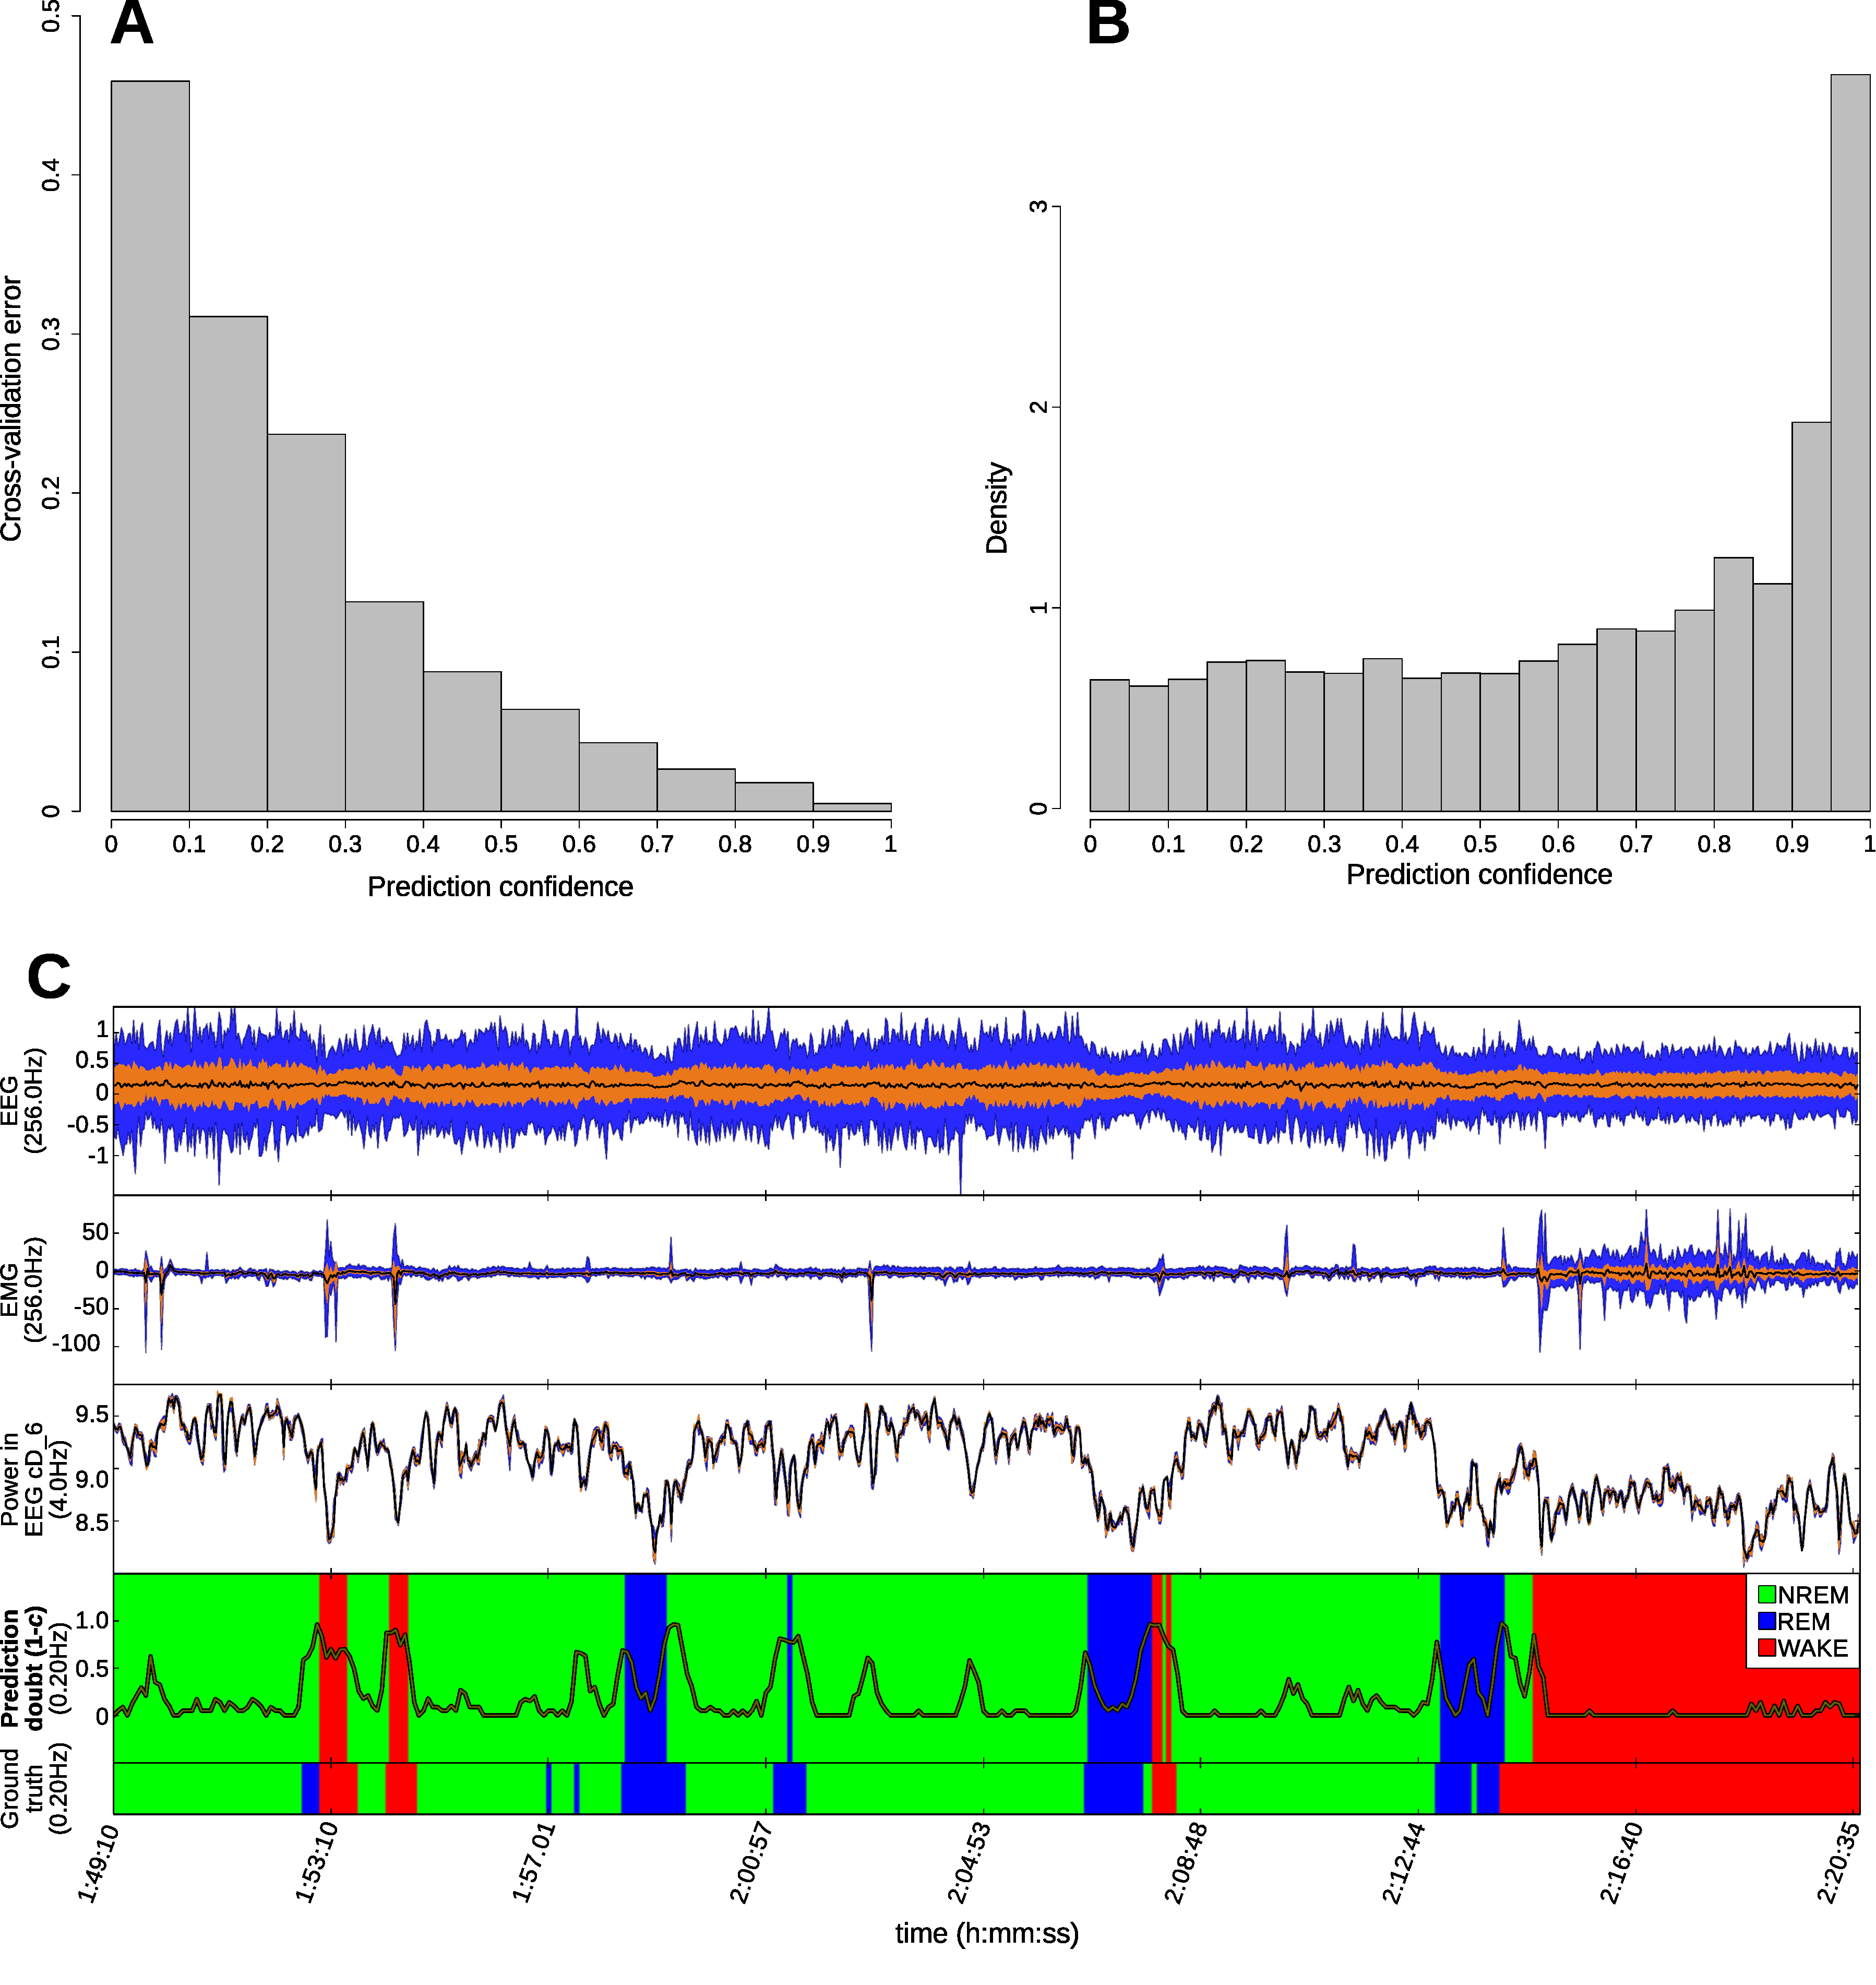
\includegraphics[width=1.0\textwidth]{figures/error.pdf}
    \caption{\ctit{A posteriori confidence assessment.}
    \textbf{A}, Relation between the confidence value derived from proportions of votes (eq.\ref{eq:entropy}) and actual proportion of error.
    Cross-validation accuracy increases with empirical confidence value.
    For low values of confidence, $[0, 0.1]$, the predictor is not very reliable (more that $45\%$ error, while random errors would be $67\%$).
    In contrast, within the highest confidence range, $(0.9, 1.0]$, misclassification are very rare($0.5 \%$).
    \textbf{B}, Distribution of confidence values for all epochs. The overall median confidence value is at 0.69.
    \textbf{C}, Visualisation of approximately 30 minutes of representative recording.
    The doubt level ($1 - c$) can be displayed on top of the prediction annotations.
    In this example, the ground truth is also displayed to illustrate cases of misclassification.
    \label{fig:error}
  }
\end{figure}
